\documentclass[tikz, border=3mm]{standalone}
\usepackage{tikz}
\usetikzlibrary{arrows.meta, decorations.markings, patterns.meta, positioning}

\begin{document}
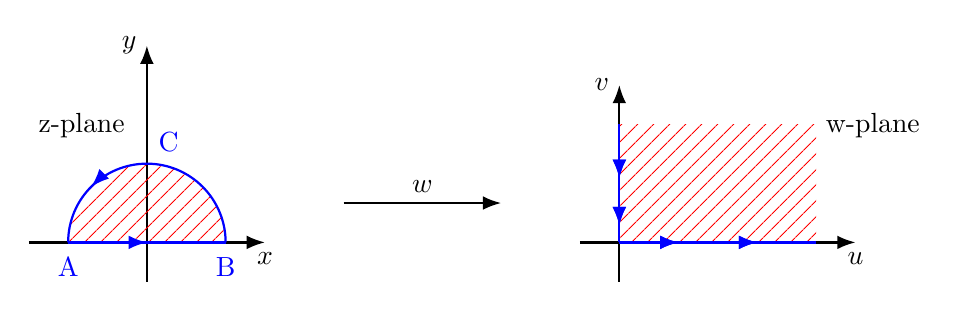
\begin{tikzpicture}[
    >=Latex, % Set default arrow tip style
    axis/.style={->, thick}, % Style for axes
    boundary/.style={blue, thick}, % Style for the boundary paths
    arrow/.style={decoration={markings, mark=at position #1 with {\arrow{>}}}, postaction={decorate}}, % Style for arrows on path
    arrow_rev/.style={decoration={markings, mark=at position #1 with {\arrow{<}}}, postaction={decorate}}, % Style for reversed arrows on path
    labelstyle/.style={blue}, % Style for labels A, B, C
    hatchstyle/.style={pattern={Lines[angle=45, distance=4pt]}, pattern color=red} % Style for hatching
]

    % --- Left Plot (z-plane) ---
    \begin{scope}
        \node[above right] at (-1.5, 1.2) {z-plane};
        % Axes
        \draw[axis] (-1.5, 0) -- (1.5, 0) node[below] {$x$};
        \draw[axis] (0, -0.5) -- (0, 2.5) node[left] {$y$};

        % Define key points and radius
        \coordinate (A) at (-1, 0);
        \coordinate (B) at (1, 0);
        \coordinate (C) at (0, 1); % Top of the arc
        \def\radius{1}

        % Fill the semi-circle region first
        \path[fill, hatchstyle] (A) -- (B) arc (0:180:\radius) -- cycle;

        % Draw boundary path A -> B with arrow
        \draw[boundary, arrow=0.5] (A) -- (B);

        % Draw boundary arc path B -> A with arrow
        \draw[boundary, arrow=0.75] (B) arc (0:180:\radius);

        % Add labels for points A, B, C
        \node[labelstyle, below=2pt of A] {A};
        \node[labelstyle, below=2pt of B] {B};
        \node[labelstyle, above right=1pt of C] {C};
    \end{scope}

    % --- Transformation Arrow ---
    \draw[->, thick] (2.5, 0.5) -- (4.5, 0.5) node[midway, above] {$w$};

    % --- Right Plot (w-plane) ---
    \begin{scope}[shift={(6,0)}] % Shift the second plot to the right
        \node[above right] at (2.5, 1.2) {w-plane};
        % Define region limits (adjust as needed)
        \def\umax{2.5}
        \def\vmax{1.5}

        % Axes
        \draw[axis] (-0.5, 0) -- (\umax+0.5, 0) node[below] {$u$};
        \draw[axis] (0, -0.5) -- (0, \vmax+0.5) node[left] {$v$};

        % Fill the rectangular region
        \fill[hatchstyle] (0,0) rectangle (\umax, \vmax);

        % Draw boundary arrows (pointing away from origin along axes)
        % Arrows on u-axis boundary
        \draw[boundary, arrow=0.3, arrow=0.7] (0,0) -- (\umax, 0);
        % Arrows on v-axis boundary
        \draw[boundary, arrow_rev=0.3, arrow_rev=0.7] (0,0) -- (0, \vmax);

    \end{scope}

\end{tikzpicture}
\end{document}